\section{Operating point and efficiency}\label{sec:efficiency}
\sectionstate{partial}{\texttt{rerun/effbudget/single/README.md} and \texttt{results/single\_track\_area.json} (chamber~A, Runs 1 and 2);
\texttt{rerun/effbudget/PASS1\_RESULT\_2026-10-31.md} (all chambers); \texttt{rerun/paper1\_ops} (scans, discharges, currents);
bookkeeping checked in \texttt{papers/paper1\_v2/figs/out/two\_particle\_numbers.md} and \texttt{NUMBERS\_RUNDOWN.md}. v2 2026-11-10:
the old sections 4 and 5.2--5.4 in three pages; one efficiency number per area; the definition, the selection variants and the
loss classes are in \cref{app:effdef}; the two-particle material is \cref{sec:twoparticle}.}
\intent{Where the chambers run and why, how efficient each is, and for the best chamber where every lost track goes.}

\subsection{What ``detected'' means}\label{sec:effdef}
The denominator is every event with one clean reference track whose ray crosses the active area of the chamber.
The muon is \emph{detected} if the chamber reconstructs a track within $R=5$\,mm of the reference ray at the mesh in
both views. When the chamber reconstructs several tracks, any of them may be the match; nothing is removed from the
denominator. The radius is the knee of the efficiency against $R$: at 5\,mm the chance that an unrelated track matches
is 0.07\,\%, and moving $R$ between 4 and 8\,mm changes the efficiency by $-0.5/{+0.7}$ percentage points, which we
quote as a systematic uncertainty (\cref{app:effdef}). For comparing chambers we also use a stricter count, in which
only the one track the reconstruction keeps may match (the \emph{kept-track} efficiency).

\subsection{Plateau and discharges}\label{sec:hvscan}
\Cref{fig:hv} shows the efficiency and the rate of discharges against $HV_\mathrm{resist}$ for four chambers. A
discharge here is a trigger in which at least one readout chip has eight or more strips above 3000 ADC counts.
\askStephan{Expected gain curve and spark behaviour for this resistivity: does what we see match production tests?}

Chamber~A reaches its plateau before discharges cost anything. Its efficiency is within one point of its maximum from
460 to 490\,V and stays between 91 and 94\,\% from 425 to 500\,V, while the fraction of reference tracks lost to a
discharge stays below 1\,\% up to 490\,V. Chamber~B behaves the same way, 10\,V higher. Chambers C and D do not reach a
plateau: at their best voltage, 480 and 430\,V, they are at 86 and 90\,\% and already lose 1.5--2.4\,\% of the tracks
to discharges, and they fall from there. The long runs of \cref{tab:datasets} were taken before the scans were
analysed, at 490--495\,V, which is 10\,V above the best voltage for chamber~A, 15\,V for B and C and 65\,V for D; at
495\,V chambers C and D lose 17 and 24\,\% of their tracks to discharges.
\askDylan{This matters for how C and D are described. At 495\,V they look like 74 and 68\,\% chambers; at their own
optimum they are 86 and 90\,\% chambers. The text now says both. D's 89.8\,\% at 430\,V is from 147 rays and it is not
verified that it uses the same half of X as its 68.0\,\% (rundown item 6).}

Two more facts about operation are documented in \cref{app:discharges}. A discharge costs no measurable dead time:
integrated over the first 0.1\,s after a discharge, the lost time is $0.2\pm0.6$\,ms for chamber~A (below 1.2\,ms at
95\,\% confidence), and compatible with zero on every chamber. And the resistive strips draw a dark current that
follows the gain, about 1\,\textmu A for chamber~A at 490\,V.

\begin{figure}[tbp]
  \centering
  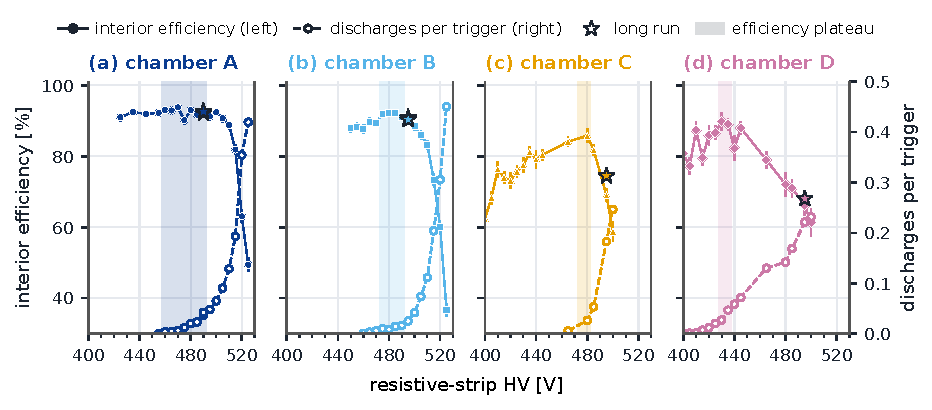
\includegraphics[width=\linewidth]{hv_scan_v2}
  \caption{Scans of $HV_\mathrm{resist}$, one chamber per panel (A on 27 June and B on 22 June at 1000\,V on the
  cathode, C and D on 26 June at 700\,V): kept-track efficiency in the interior (left axis, solid) and discharges per
  trigger (right axis, dashed, open). Shaded: the efficiency plateau, within one point of the maximum. Stars: the long
  runs. Chamber~C's long run was taken on the morning of 26 June, before its scan, while the gas was still drying; it
  lost fewer tracks to discharges and lies above the scan. Chamber~E has no scan. About 4\,\% of all triggers of
  chamber~A carry a discharge at 490\,V, but only 0.9\,\% of its reference tracks are lost to one.}
  \label{fig:hv}
\end{figure}

\subsection{Five chambers}\label{sec:fleet}
\Cref{fig:effmap} maps the efficiency of the five chambers. Chambers A and B are uniform over their active area. The
other three show the production defects that the rest of this paper leaves aside: whole-plane discharges on chambers C
and D, a fault of the X readout on half of chamber~D, and stripes of chamber~E that do not amplify
(\cref{app:beam}). In the interior and at the voltage of the long runs, the kept-track efficiency is 92.3\,\% for
chamber~A, 90.3\,\% for B, 74.4\,\% for C, 68.0\,\% for D (on the good half of its X readout) and 40.9\,\% for E
(71.3\,\% in its live bands). No single loss class takes more than 1.7\,\% of the tracks of chambers A and B.

\begin{figure}[tbp]
  \centering
  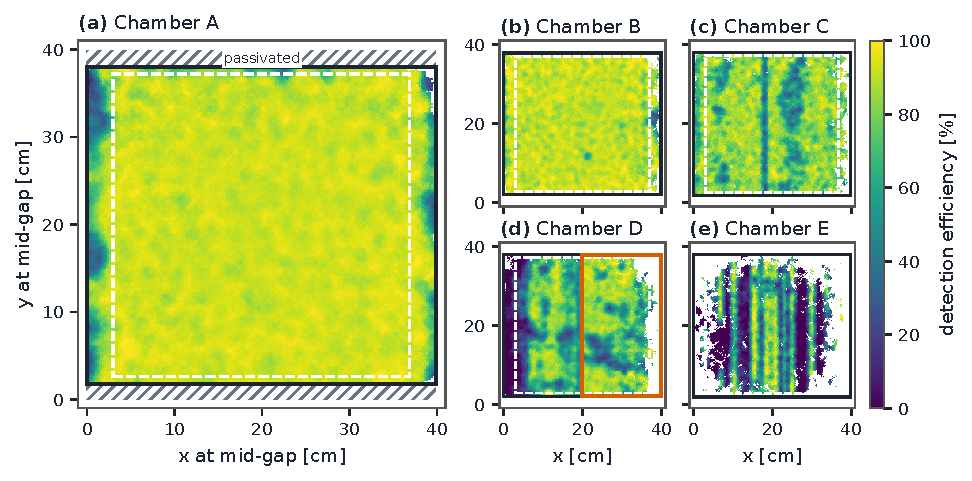
\includegraphics[width=0.92\linewidth]{efficiency_map}
  \caption{Kept-track efficiency maps of the five chambers (8\,mm disk on a 2\,mm grid; axes in cm), on one scale.
  Each map pools all runs of its chamber within 3 points of the efficiency of its long run, at the drift field of that
  run: for chamber~A 30 runs and scan points with 70\,470 reference rays, of which Runs 1 and 2 are two; for C and D
  the pool includes scan points at lower voltage. Solid box: active area; white dashed: interior; hatched on (a): the
  passivated strip ends, outside the active area. (d) Chamber~D: a fault of the X readout affects channels 0--255, so
  only the right half (orange box) is quoted. Blank: outside the active area or fewer than 15 rays.}
  \label{fig:effmap}
\end{figure}

\subsection{Chamber A: single-track efficiency and where the loss goes}\label{sec:single}
To ask how efficient the chamber is for one track, events with a second particle in the chamber have to be set
aside without letting the chamber's own failures decide which events those are: a failure that looks like two tracks
would otherwise remove itself from the sample. The reference telescope cannot do it, because second particles are
mostly local, soft secondaries. We use the two views instead. A real second particle is ionisation in the gas, seen in
both views with the same charge (\cref{sec:balance}); an event leaves the single-track sample only if it carries such a
second particle (\cref{sec:twoeff}). Everything else stays and counts against the chamber. Of the 29\,398 reference
tracks of Runs 1 and 2, 931 come with a second particle and 28\,467 are single tracks.

The single-track efficiency of chamber~A is
\[ \varepsilon=94.8\pm0.1\,\text{(stat)}\,^{+0.7}_{-0.5}\,(R)\ \%\]
over the full active area, and 95.7\,\% in the interior. \Cref{fig:lossbudget} shows where the missing 5.2\,\% goes.

\emph{The chamber itself: 0.6\,\%.} Discharges (0.47\,\%) and noise bands, patches of strips with a shifted baseline
(0.10\,\%), are the only losses that belong to the hardware.

\emph{$\delta$-rays: 2.4\,\%.} The largest group is a muon accompanied by its own knock-on electron, which the
straight-track reconstruction does not describe (\cref{sec:straight}).

\emph{The edges: 0.9 points.} Within 30\,mm of the unpassivated $x$ sides the drift field fringes
(\cref{sec:edge}); tracks there spread over more strips or are fitted off. This is the difference between the full
area and the interior.

\emph{The rest: 0.7\,\%.} Fits that are off with nothing flagged (0.34\,\%), second deposits that are not
particle-like (0.18\,\%) and tracks with the right angle more than 5\,mm from the reference (0.16\,\%), of which
about two thirds are muons that scattered between the reference planes.

All but 0.6 points of the inefficiency is therefore real ionisation that the reconstruction does not yet handle. Every
loss class, with an event display and the result of trying to recover it, is in \cref{app:effdef}.

\begin{figure}[tbp]
  \centering
  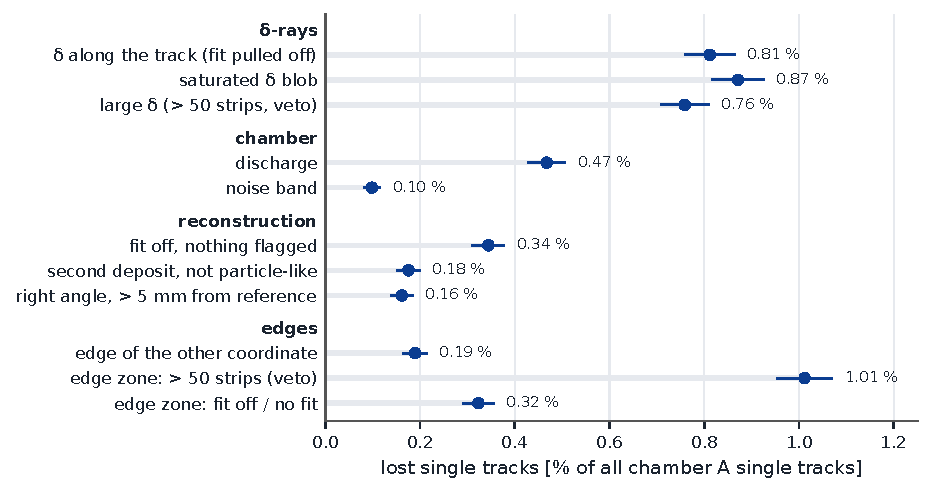
\includegraphics[width=0.82\linewidth]{loss_budget}
  \caption{Where the single-track inefficiency of chamber~A goes, over the full active area (Runs 1 and 2, 28\,467
  single-track reference tracks, 5.2\,\% lost), by class with Poisson errors. The group ``edges'' counts every track
  lost in the edge zone, including about 0.4 points that those tracks would lose at the rate of the interior; the cost
  of the edges proper is the 0.9 points between the full-area and the interior efficiency.}
  \label{fig:lossbudget}
\end{figure}
